\documentclass[12pt]{beamer}
\usetheme{AnnArbor}
\usecolortheme{crane}
%\usetheme{Berlin}
%\usecolortheme{wolverine}

\setbeamertemplate{background canvas}[vertical shading][top=magenta!0,bottom=cyan!0]

\setbeamercolor{block title example}{bg=pink}
\usepackage{url}
\usepackage{chapterbib}
\usepackage{hyperref} 

 \usepackage{multicol}
% \usepackage{pgf,pgfarrows,pgfnodes}
% \usepackage{verbatim} 
%\usepackage{comment}
%\usepackage{multirow}
% \usepackage{graphics}
% \usepackage{graphicx}
% \usepackage{tikz}
%\usepackage{pgfplots}
%Basic Information
\renewcommand{\bibname}{References}

\newcommand\Fontvi{\fontsize{10}{7.2}\sffamily}
\newcommand\FontviAuth{\fontsize{12}{7.2}\sffamily}
\newcommand\FontviRef{\fontsize{6}{7.2}\sffamily}
\newcommand\FontviHead{\fontsize{25}{10}\sffamily}


\title{Enhacement of JMeter}
%\author{ 
% \begin{minipage}[t]{0.48\linewidth}
%   \begin{flushright}
%   Buddha Sushmitha \\
%   Dhruv Joshi\\
%   Manisha Choudhury \\
%   Naman Choudhary \\
%   Shekhar Saurav \\
%   Surabhi Mour \\
%   \end{flushright}
% \end{minipage}
% \begin{minipage}[t]{0.48\linewidth}
%   \begin{flushleft}
%  KIET \\
%  NIT Rourkela\\
%  NIT Rourkela \\
%  NIT Jamshedpur \\
%  NIT Jamshedpur\\
%  SVNIT Surat \\
% \end{minipage}


 
%}
%\author{B. Sushmitha\hskip50pt KIET\\  Dhruv Joshi \hskip45pt NIT Rourkela\\ Manisha Choudhury\hskip10pt NIT Rourkela\\ Naman Choudhary\hskip34pt NIT Jamshedpur \\  Shekhar Saurav \hskip42pt  NIT Jamshedpur \\ Surabhi Mour\hskip40pt SVNIT Surat}
\author[JMeter Team]{\FontviAuth{\hspace{0.3cm} B. Sushmitha \hspace{1cm} Dhruv Joshi \hspace{1cm} Manisha Choudhury} \\
				\vspace{0.2cm} \Fontvi{\hspace{0.3cm} KIET \hspace{1.1cm} NIT Rourkela \hspace{1.2cm} NIT Rourkela} \\
				\vspace{0.8cm}\FontviAuth{Naman Choudhary \hspace{1cm} Shekhar Saurav \hspace{1cm} Surabhi Mour}\\\vspace{0.2cm} 
				\Fontvi{\hspace{0.3cm}NIT Jamshedpur \hspace{1.3cm} NIT Jamshedpur \hspace{1.2cm} SVNIT Surat}}
%\institute{KIET \\ SVNIT Surat \\ NIT Rourkela \\ NIT Jamshedpur  }
\date{03 July 2013}
%
\logo{\flushbottom
\includegraphics[width=2.5cm, height=1cm]{images/logo1}}
\usebackgroundtemplate{
\includegraphics[width=\paperwidth]{images/background1.png}}
%--------------------------------------------------------------------------------------
%               TITLE PAGE (Slide 1)
%--------------------------------------------------------------------------------------
\begin{document}
\vspace{0.5cm}
\begin{frame}
\titlepage

\includegraphics[width=1.2cm, height=1.2cm]{images/logos/nitr_logo} \hspace{0.5cm}

\includegraphics[width=1.2cm, height=1.2cm]{images/logos/nitsurat_logo} \hspace{0.5cm}

\includegraphics[width=1.5cm, height=1.5cm]{images/logos/IITB_logo} \hspace{0.5cm}

\includegraphics[width=1.2cm, height=1.2cm]{images/logos/kiet_logo} \hspace{0.5cm}

\includegraphics[width=1.0cm, height=1.2cm]{images/logos/nitjsr_logo} \hspace{1cm}
\end{frame}
%--------------------------------------------------------------------------------------

\section{Guides}
\begin{frame}
 \frametitle{Our Guides}
  \textbf{Principle Investigator}\\
  \hspace{0.2cm}Prof. D. B. Phatak\\
  \vspace{0.5cm}
  \textbf{Project In-Charge}\\
  \hspace{0.2cm}Mr. Nagesh Karmali\\
  \vspace{0.5cm}
  \textbf{Mentors}\\
  \hspace{0.2cm}Miss. Silpa T.\\
  \hspace{0.2cm}Miss Firuza Aibara\\
  \hspace{0.2cm}Mr. Sukhdeo Gupta
  
\end{frame}



% %--------------------------------------------------------------------------------------
% %               Outline
% %--------------------------------------------------------------------------------------
% \begin{frame}
% \frametitle{Outline}
% \begin{multicols}{2}
% \tableofcontents
% %\tableofcontents[hideallsubsections]
% \end{multicols}
% \end{frame}
% %--------------------------------------------------------------------------------------
\section{Introduction}
\begin{frame}
 \begin{center}
    \FontviHead{INTRODUCTION}
 \end{center}

 
\end{frame}


\subsection{}
\begin{frame}[c]
\frametitle{Why do we use  JMeter?}
Considering a typical web-application, we could have 1000s of users trying to access it concurrently. We may not choose to employee 1000 testers for every such user for performance evaluation of the application.
\\
\begin{center}
	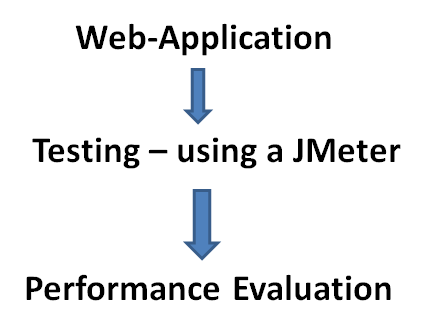
\includegraphics[width=6cm, height=4.5cm]{images/flow.png}
\end{center}
\end{frame}

%--------------------------------------------------------------------------------------
%               Slide 2
%--------------------------------------------------------------------------------------
\subsection{}
\begin{frame}[c]
\frametitle{More on Testing}
Testing Parameters:
\begin{itemize}
\item User
\item Data
\item Time
\end{itemize}
Performance testing Comprises of:
\begin{enumerate}
\item Load Testing
\item Stress Testing
\item Scalability Testing
\end{enumerate}
and calculating Response Time, Latency, Throughput and other such Metrics.
\end{frame}

 
%--------------------------------------------------------------------------------------
%               Slide 3
%--------------------------------------------------------------------------------------
\subsection{}
\begin{frame}[c]
\frametitle{A sample JMeter 'TESTPLAN'}
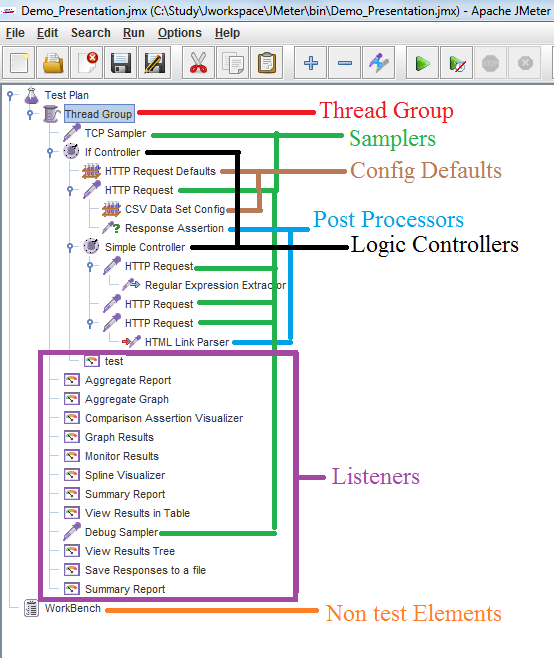
\includegraphics[width=9cm, height=7.5cm]{images/testplan.png}
\end{frame}

%--------------------------------------------------------------------------------------
%               Slide 4
%--------------------------------------------------------------------------------------
\section{Some JMeter Plugins}
\begin{frame}[c]
\frametitle{Some JMeter Plugins}
  \begin{itemize}
    \item \textbf{Thread group Plugins}
	\begin{itemize}
	\item Stepping Thread Group
	\item Ultimate Thread Group
	\end{itemize}
   \item \textbf{Timeline Graph Plugins}
	\begin{itemize}
	\item Active Threads Over Time
	\item Response Times Over Time
	\item Response Latency Over Time
	\item Transactions per Second
	\item Server Hits per Seconds
	\item Bytes Throughput Over Time
	\end{itemize}
  \end{itemize}
\end{frame}

%--------------------------------------------------------------------------------------
%               Slide 5
%--------------------------------------------------------------------------------------
\section{Enhancements}
\begin{frame}[c]
\frametitle{JMeter Enhancements Implemented}
	\begin{itemize}
	 \item<+-|alert@+> \textbf{Dynamic Bandwidth Throttling}\\
	  for the requests being sent, based on response error percentage
	 \item<+-|alert@+> \textbf{IP Spoofing}\\
	  distinct IP addresses for each virtual user
	\item<+-|alert@+> \textbf{Auto CSV Generation}\\
	  creating A .csv file directly from the database table mentioned
	\item<+-|alert@+> \textbf{Automating TPC-C Testing}\\
	  Test script for Oracle and MySQL that enables a tester to carry out preliminary TPCC testing
	\end{itemize}
\end{frame}

%--------------------------------------------------------------------------------------
%               Slide 6
%--------------------------------------------------------------------------------------
\subsection{}
\begin{frame}[c]
	\begin{itemize}
	 \item<+-|alert@+> \textbf{Filtered Results Table}\\
	  Filters the sampler results, based on user specified parameters
	\item<+-|alert@+> \textbf{Constant Increasing Timer}\\
	  Stepping Up time interval between Samples requested
	\item<+-|alert@+> \textbf{Enhanced Assertion results}\\
	Details of the Sampler passing or failing the test
	\item<+-|alert@+> \textbf{SMTP Defaults}\\
	  A configuration element for setting data for SMTP Samplers under it
	
	\end{itemize}
\end{frame}

%--------------------------------------------------------------------------------------
%               Slide 7
%--------------------------------------------------------------------------------------
\section{AutoCSV Generation}
\begin{frame}
 \begin{center}
    \FontviHead{AutoCSV Generation}
 \end{center}

 
\end{frame}
% \section{Slide Title7}
% \begin{frame}[c]
% 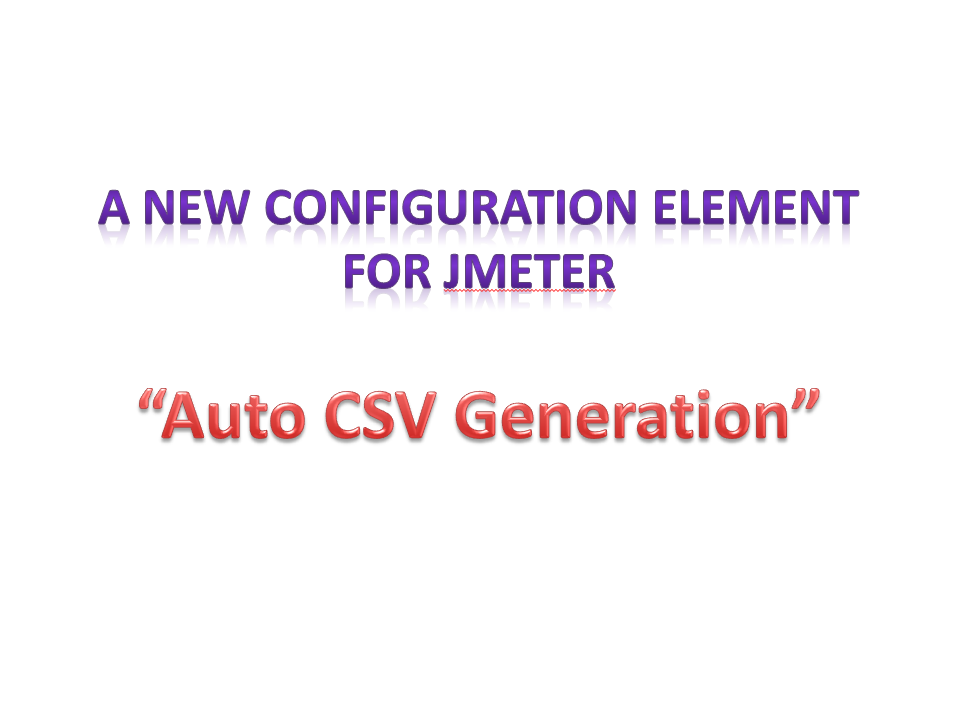
\includegraphics[width=12cm, height=8cm]{images/autocsv.png}
% \end{frame}

%--------------------------------------------------------------------------------------
%               Slide 8
%--------------------------------------------------------------------------------------
\subsection{Application to be tested}
\begin{frame}[c]
\frametitle{Application to be tested}
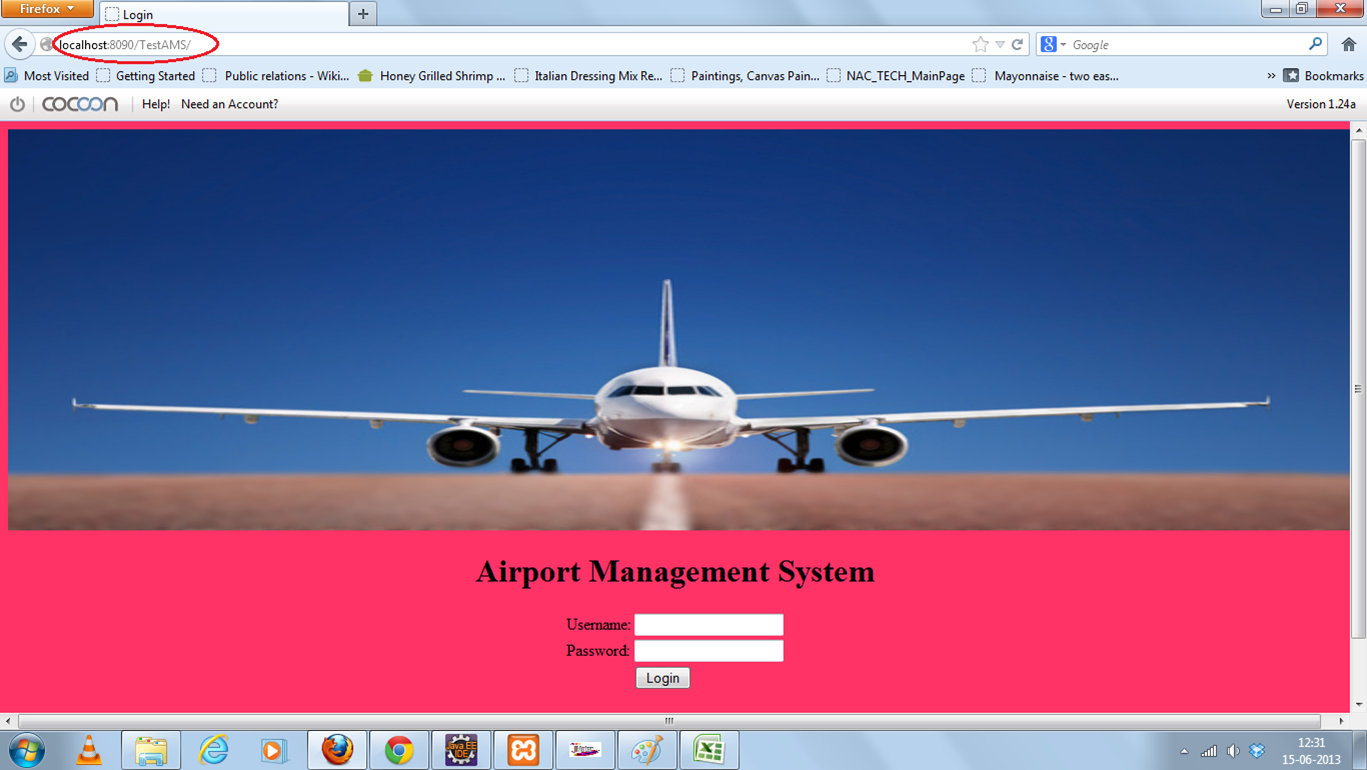
\includegraphics[width=12cm, height=7.5cm]{images/ams.png}
\end{frame}

%--------------------------------------------------------------------------------------
%               Slide 9
%--------------------------------------------------------------------------------------
\subsection{The Auto CSV Generation GUI}
\begin{frame}[c]
\frametitle{The Auto CSV Generation GUI}
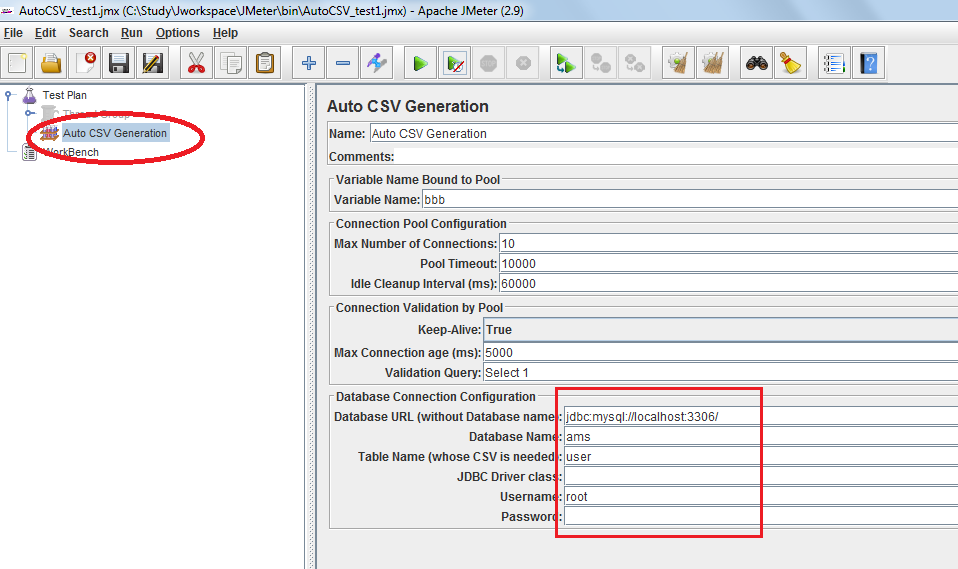
\includegraphics[width=12cm, height=7.5cm]{images/autocsvgui.png}
\end{frame}

%--------------------------------------------------------------------------------------
%               Slide 10
%--------------------------------------------------------------------------------------
\subsection{The .csv file generated in /bin folder}
\begin{frame}[c]
\frametitle{The .csv file generated in /bin folder}
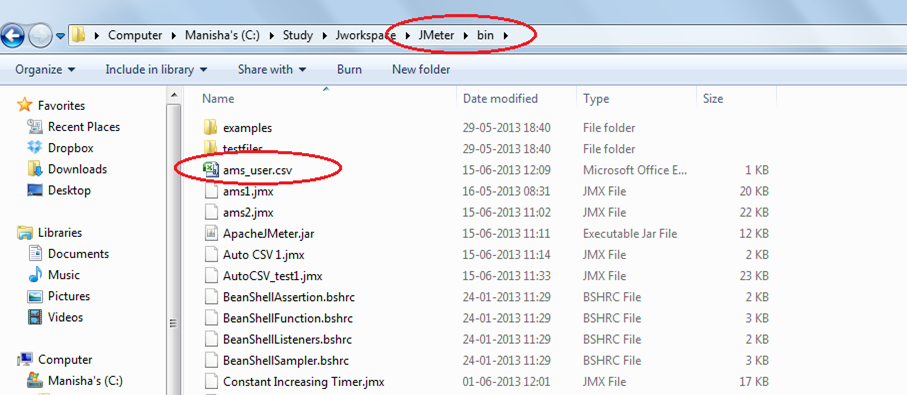
\includegraphics[width=12cm, height=7.5cm]{images/csvfile.png}
\end{frame}

%--------------------------------------------------------------------------------------
%               Slide 11
%--------------------------------------------------------------------------------------
\subsection{The ams\_user.csv generated}
\begin{frame}[c]
\frametitle{The ams\_user.csv generated}
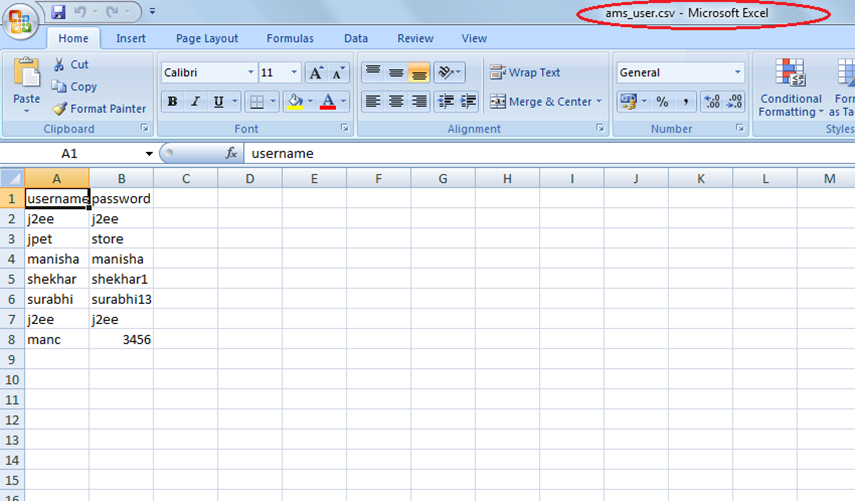
\includegraphics[width=12cm, height=7.5cm]{images/csv.png}
\end{frame}

%--------------------------------------------------------------------------------------
%               Slide 12
%--------------------------------------------------------------------------------------
\subsection{}
\begin{frame}[c]
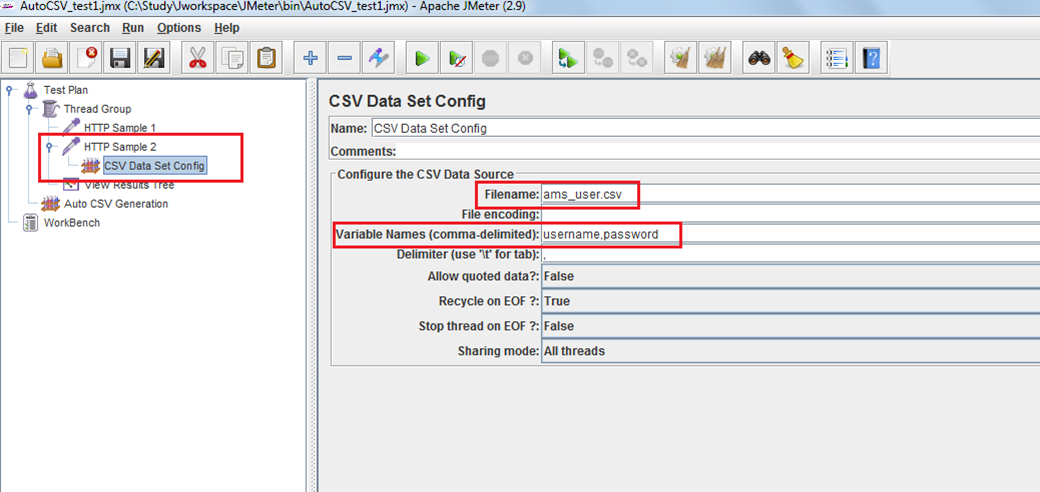
\includegraphics[width=12cm, height=7.5cm]{images/testplancsv.png}
\\The “CSV data config” element is added as child of HTTP Sampler
\end{frame}

%--------------------------------------------------------------------------------------
%               Slide 13
%--------------------------------------------------------------------------------------
\subsection{}
\begin{frame}[c]
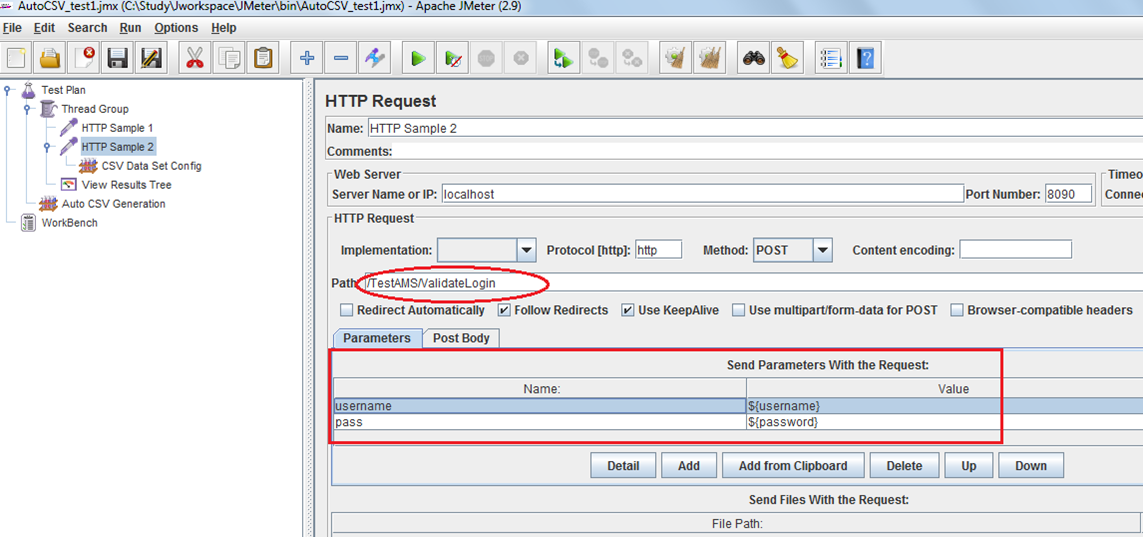
\includegraphics[width=12cm, height=7.5cm]{images/testplancsv2.png}
\\The HTTP sampler where the parameters of .csv file are set
\end{frame}

%--------------------------------------------------------------------------------------
%               Slide 14
%--------------------------------------------------------------------------------------
\subsection{}
\begin{frame}[c]
\frametitle{Output - CSV data verification}
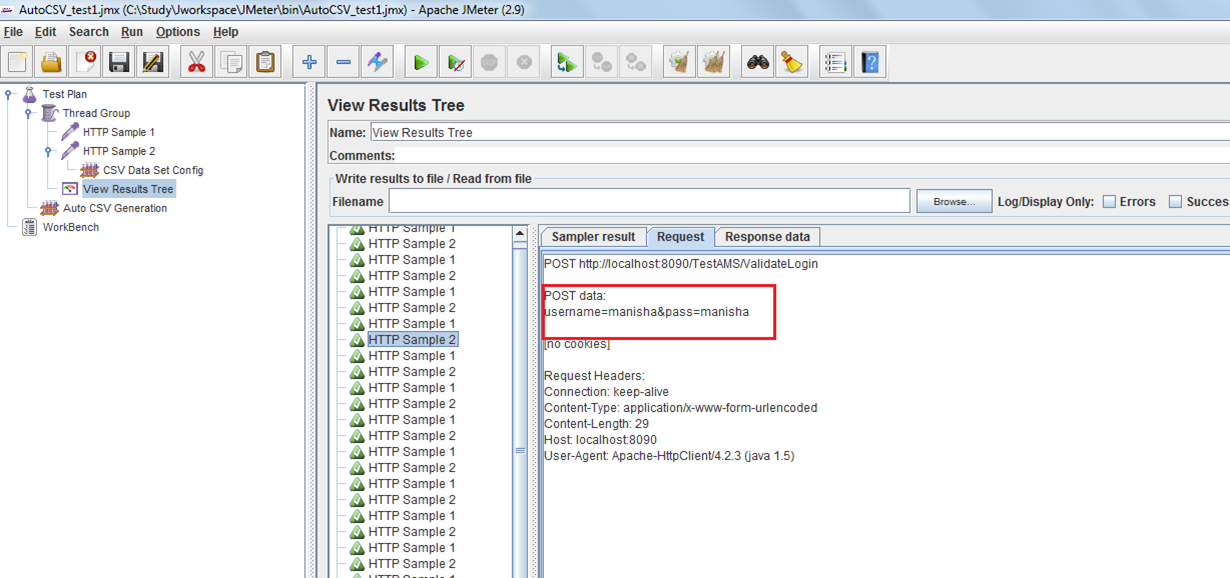
\includegraphics[width=12cm, height=7.5cm]{images/obs.png}
\end{frame}




%--------------------------------------------------------------------------------------
%               Slide 1a
\section{Bandwidth Throttling}
\begin{frame}
 \begin{center}
    \FontviHead{Bandwidth Throttling}
 \end{center}

 
\end{frame}

%--------------------------------------------------------------------------------------
\section{Bandwidth Throttling}
\begin{frame}[c]
\frametitle{Bandwidth Throttling}
  			\begin{itemize}
				\item<+-|alert@+>Bandwidth throttling is the intentional slowing of Internet service. \\
				\item<+-|alert@+>In real world scenario, people use different web services  at different bandwidths. \\

% 				\begin{itemize}
% 					\item<+->Genetics
% 					\item<+->Medicine
% 					\item<+->Bioinformatics
% 					\item<+->Saptial data mining
% 					\item<+->Education
% 				\end{itemize}\pause
				\item<+-|alert@+> Using Bandwidth Throttling, JMeter can be used to create test plans to simulate slower connections.

			\end{itemize}

\end{frame}

\subsection{User Interface}
\begin{frame}[c]

\frametitle{User Interface}
 \begin{itemize}
  \item<+-| alert@+> To use bandwidth throttling in JMeter, a gui component has been added to HTTP Request Defaults Config Element.\\
  \vspace{1cm}
  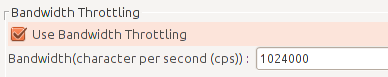
\includegraphics[width=10cm, height=2cm]{images/bt1}
 \end{itemize}
\end{frame}

\subsection{Working of Bandwidth Throttling in JMeter}
\begin{frame}[c]
\frametitle{Test Plan}
\begin{minipage}[t]{0.48\linewidth}
  \begin{itemize}
   \item Thread groups : 2\\
   \item Thread count : 5  \\
   \item Loop count  : 5 \\
   \item HTTP Samplers : 1 \\
  \end{itemize}
  \end{minipage}\hfill
  \begin{minipage}[t]{0.48\linewidth}
    \vspace{-1cm}
    \centering{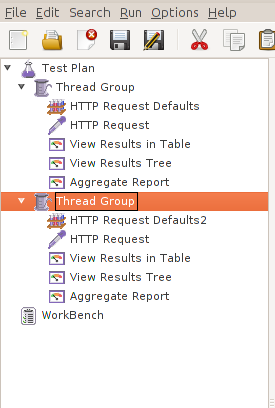
\includegraphics[width=4cm, height=6cm]{images/bt2}}

    \end{minipage}

\end{frame}

\begin{frame}[c]
 \frametitle{HTTP Default Settings for Samplers}
 \begin{minipage}[t]{0.48\linewidth}
  \centering
   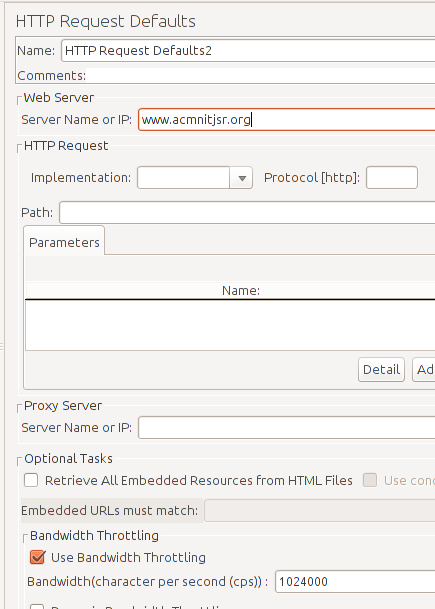
\includegraphics[width=5cm, height=7.5cm]{images/bt3}
 \end{minipage}
 \begin{minipage}[t]{0.48\linewidth}
  \centering
    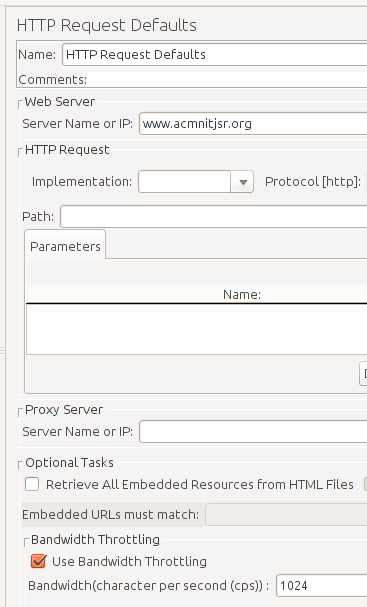
\includegraphics[width=5cm, height=7.5cm]{images/bt4}
 \end{minipage}

 \end{frame}

 \subsection{Test Results}
 \begin{frame}[c]
  \frametitle{Result Table for Thread group 1}
  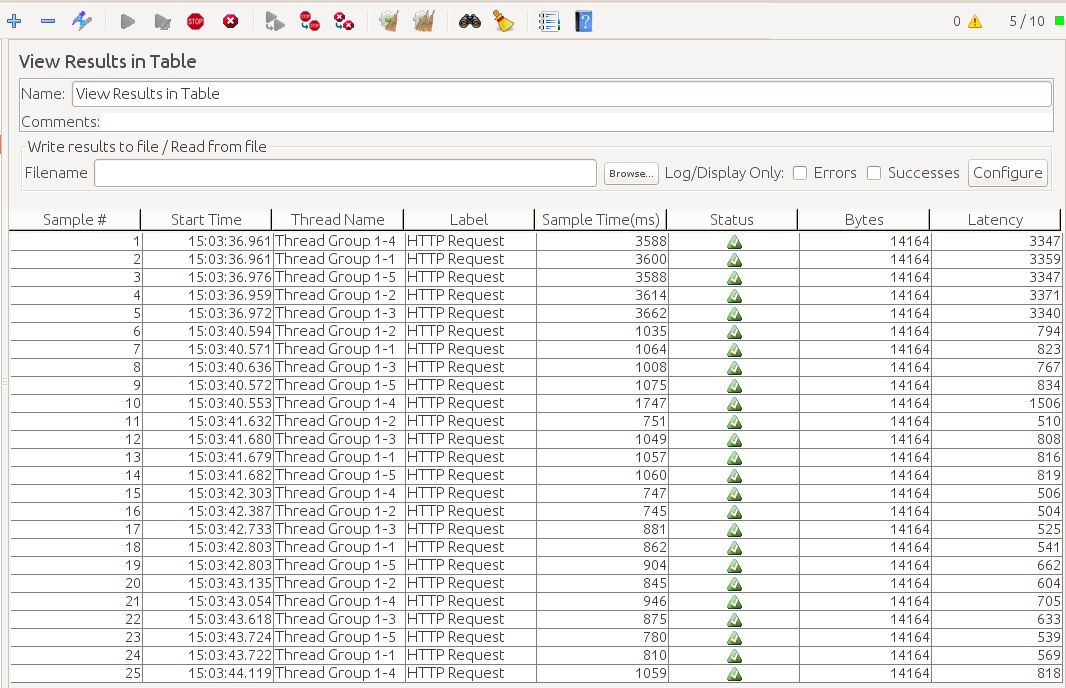
\includegraphics[width=12cm, height=7.5cm]{images/bt5}
 \end{frame}
 
  \begin{frame}[c]
  \frametitle{Result Table for Thread group 2}
  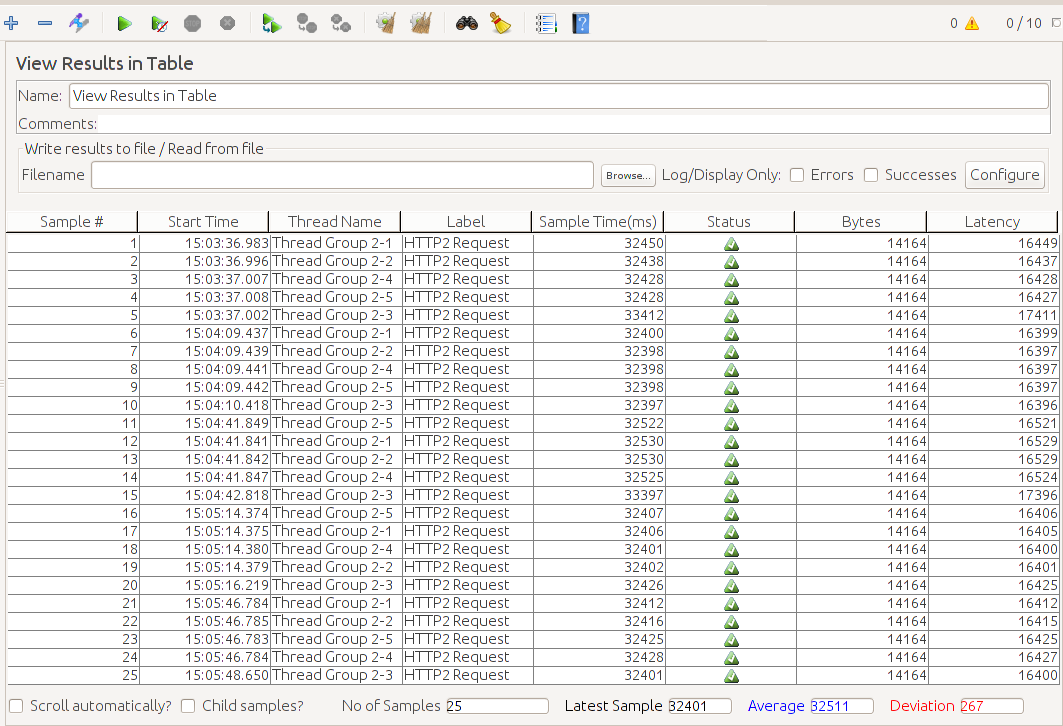
\includegraphics[width=12cm, height=7.5cm]{images/bt6}
 \end{frame}

 \begin{frame}[c]	
 \frametitle{Results Comparison}
 \begin{minipage}[t]{0.48\linewidth}
 Bandwidth: 1MBps\\
  \centering
   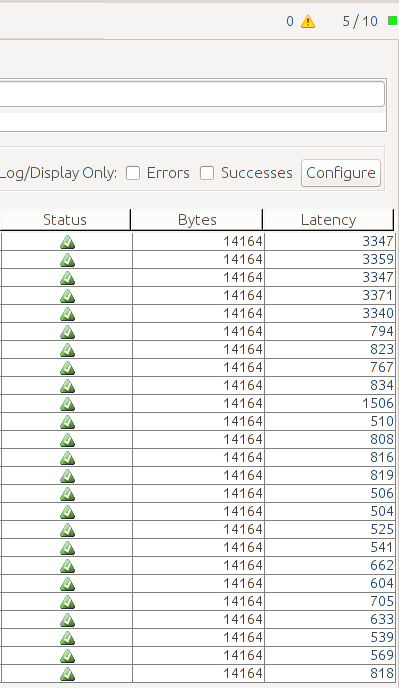
\includegraphics[width=5cm, height=7.5cm]{images/bt7}
 \end{minipage}
 \begin{minipage}[t]{0.48\linewidth}
  \centering
  Bandwidth: 1KBps
   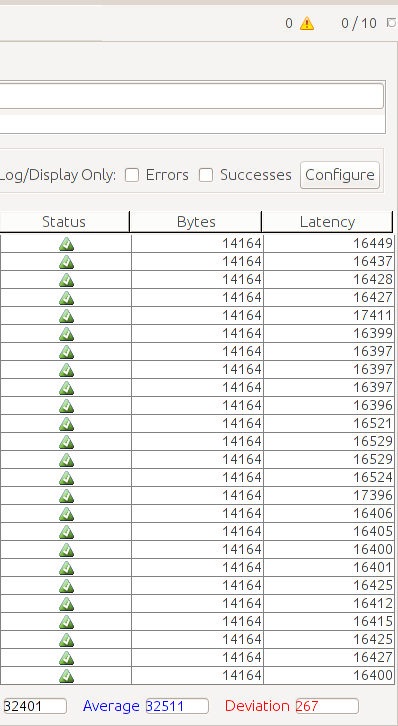
\includegraphics[width=5cm, height=7.5cm]{images/bt8}
 \end{minipage}

 \end{frame}
 
  \begin{frame}[c]	
 \frametitle{Aggregate Reports}
Bandwidth: 1MBps\\
   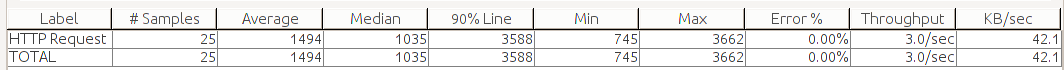
\includegraphics[width=12cm, height=1.2cm]{images/bt10}\\
\vspace{1cm}
Bandwidth: 1KBps
   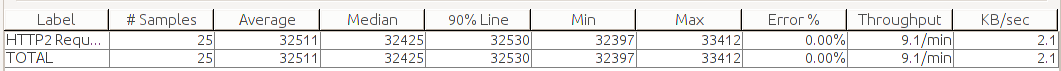
\includegraphics[width=12cm, height=1.2cm]{images/bt9}\\
 

 \end{frame}


%--------------------------------------------------------------------------------------
%               Slide 2
\section{Dynamic Bandwidth Throttling}
\begin{frame}
 \begin{center}
    \FontviHead{Dynamic Bandwidth Throttling}
 \end{center}

 
\end{frame}

%--------------------------------------------------------------------------------------
\section{Dynamic Bandwidth Throttling}
\begin{frame}[c]
\frametitle{Dynamic Bandwidth Throttling}
\begin{enumerate}
 \item <+-| alert@+>DBT deals with the variation of bandwidth at runtime.
 \item <+-| alert@+>DBT can be used to test performance of web services under varying bandwidth (load).
 \item <+-| alert@+>DBT can be used to measure and manage errors during the test at runtime.
 \item <+-| alert@+>Based on error rate.
 \item <+-| alert@+>A distributed testing can be simulated using DBT and IP spoofing.
\end{enumerate}

% 
% \begin{enumerate}
% \item Point 1
% \item Point 2 \cite{Features}
% \item Point 3
% \begin{itemize}
% \item Point a
% \item Point b
% \end{itemize}
% \item Point 4
% \end{enumerate}
 \end{frame}
 
 \subsection{User Interface}
  \begin{frame}[c]
    \frametitle{User Interface}
    \begin{flushleft}
     
    To use Dynamic Bandwidth Throttling in JMeter, an extended GUI component has been added to Bandwidth Throttling in HTTP Request Defaults.
    \end{flushleft}

     \centering
    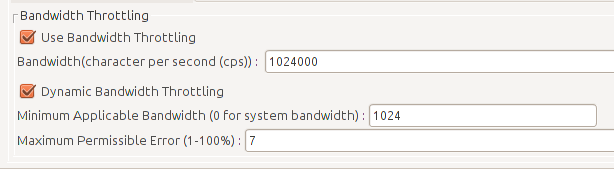
\includegraphics[width=10cm, height=3.5cm]{images/dbt1}
       
  \end{frame}
  
  \subsection{Working of Dynamic Bandwidth Throttling}
   \begin{frame}
   \frametitle{Test Plan}

\begin{minipage}[t]{0.48\linewidth}
  \begin{itemize}
        \item Thread Group: 1
        \item Thread Count: 1000
        \item Ramp Up period: 0 sec
        \item Timeout period: 22 sec
        \item No. of Samplers: 11
        \item Permisibble error: 7\%
        \item Applicable bandwidth: 1MBps
        \item Minimum applicable bandwidth: 1KBps
  \end{itemize}
  \end{minipage}\hfill
  \begin{minipage}[t]{0.48\linewidth}
    \vspace{-1cm}
    \centering{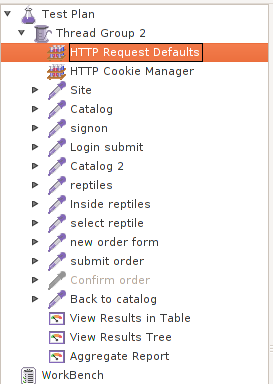
\includegraphics[width=5cm, height=7.5cm]{images/dbt2}}

    \end{minipage}
   \end{frame}

  \subsection{Test Results}
  \begin{frame}
    \frametitle{Aggregate Report}
    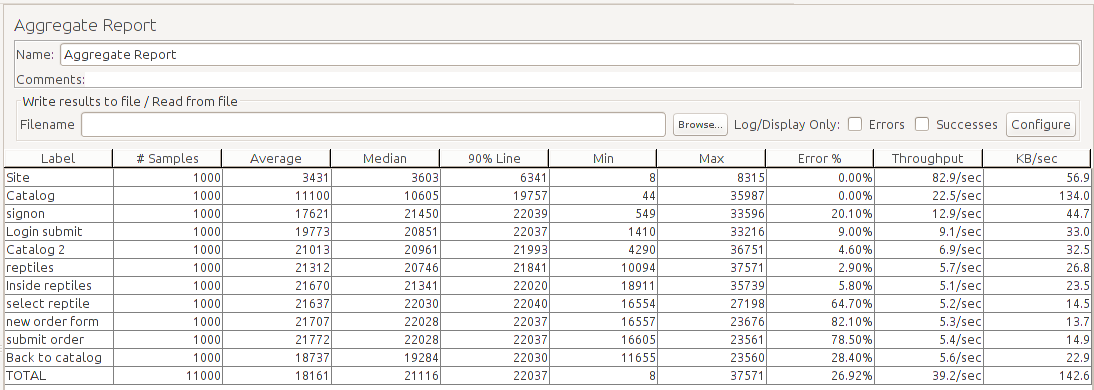
\includegraphics[width=12cm, height=7.5cm]{images/dbt3}
    
  \end{frame}
  
    \begin{frame}
    \frametitle{Aggregate Report}
    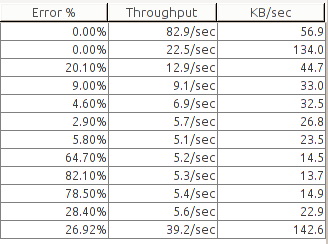
\includegraphics[width=12cm, height=7.5cm]{images/dbt4}
    
  \end{frame}

  \subsection{JMeter Log Report}
    \begin{frame}
      \frametitle{JMeter Log Report}
      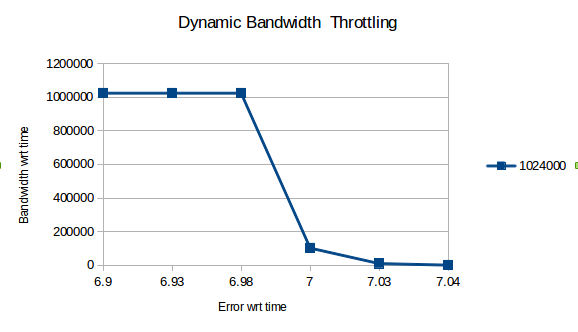
\includegraphics[width=12cm, height=8cm]{images/dbt6}
      
    \end{frame}
    
    \subsection{JMeter Log Report}
    \begin{frame}
      \frametitle{JMeter Log Report}
      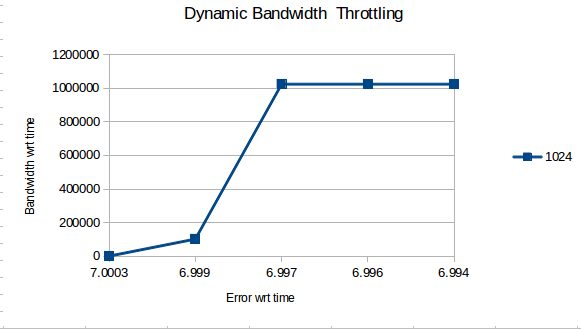
\includegraphics[width=12cm, height=8cm]{images/dbt5}
      
    \end{frame}


%--------------------------------------------------------------------------------------
%               Slide 1a

\section{IP Spoofing}
\begin{frame}
 \begin{center}
    \FontviHead{IP Spoofing}
 \end{center}

 
\end{frame}

%--------------------------------------------------------------------------------------
\subsection{What is IP address Spoofing?}
\begin{frame}[c]
\frametitle{What is IP address Spoofing?}
It is the creation of IP Packets with forged source IP address, with the purpose of concealing identity of the sender or for impersonating another computer system.
\end{frame}

%--------------------------------------------------------------------------------------
%               Slide 2
%--------------------------------------------------------------------------------------
\subsection{IP Spoofing in JMeter}
\begin{frame}[c]
\frametitle{IP Spoofing in JMeter}
\begin{enumerate}
\item JMeter is capable of generating thousands of threads that act as virtual users
\item On the server side, these requests appear from the same IP address on which JMeter resides
\item On servers which have IP dependent response, the testplan with a thousand virtual fails
\item To eliminate this drawback, we use IP Spoofing in JMeter
\end{enumerate}
 \end{frame}

 
%--------------------------------------------------------------------------------------
%               Slide 3
%--------------------------------------------------------------------------------------
\subsection{}
\begin{frame}[c]
\frametitle{Without IP spoofing}
Load balancing inactive
\begin{figure}
 \centering
 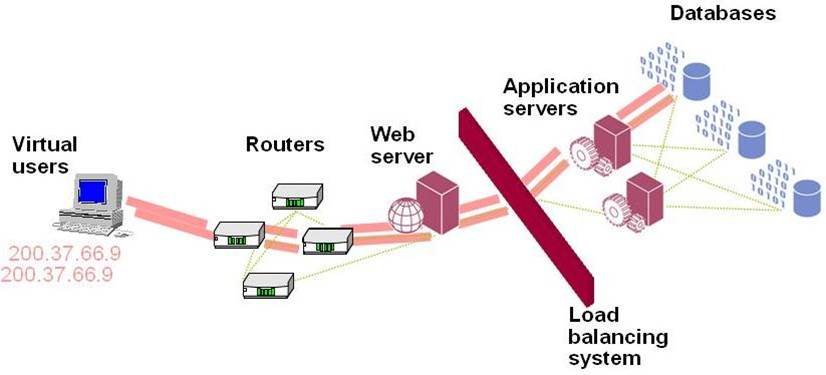
\includegraphics[width=12cm]{images/woip.jpg}
 \caption{Server treating multiple requests without IP spoofing}
\end{figure}
\end{frame}


%--------------------------------------------------------------------------------------
%               Slide 4
%--------------------------------------------------------------------------------------
\subsection{}
\begin{frame}[c]
\frametitle{With IP spoofing}
Load balancing active
\begin{figure}
 \centering
 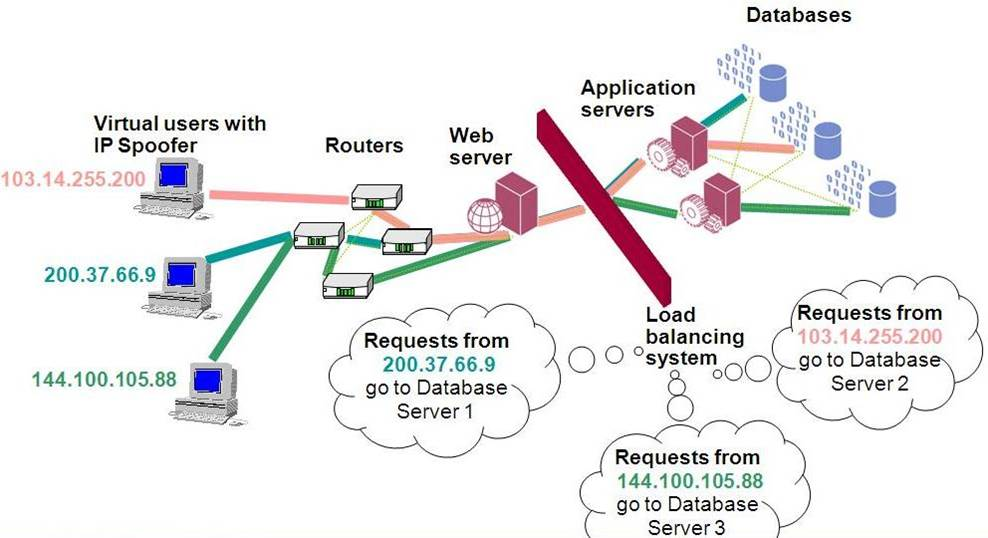
\includegraphics[width=12cm]{images/wip.jpg}
 %Move this photo up as the caption is getting hidden
 \caption{Server treating multiple requests with IP spoofing}
\end{figure}
\end{frame}


%--------------------------------------------------------------------------------------
%               Slide 5
%--------------------------------------------------------------------------------------
\subsection{JMeter Implementation}
\begin{frame}[c]
\frametitle{JMeter Implementation}
  \begin{block}{IP and Subnet Details}
	We need to provide JMeter with IP address of the machine and the subnet it belongs to, and also specify the number of IP addresses required
  \end{block}
  \begin{block}{IP allocation}
	JMeter internally allocates virtual IPs to the same machine, and each virtual user can send request from a distinct IP from newly allocated virtual IPs
  \end{block}
\end{frame}

%--------------------------------------------------------------------------------------
%               Slide 6
%--------------------------------------------------------------------------------------
\subsection{Interface of IP Spoofing Config Element in JMeter}
\begin{frame}[c]
\frametitle{Interface of IP Spoofing Config Element in JMeter}
\begin{figure}
 \centering
 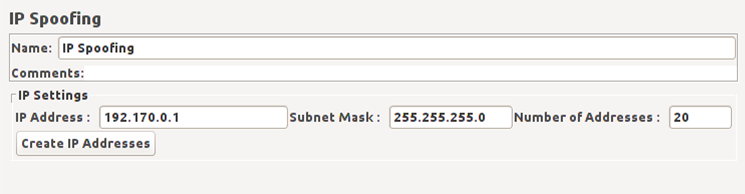
\includegraphics[width=12cm]{images/interface.png}
 \caption{GUI of IP Spoofing}
\end{figure}
\end{frame}

%--------------------------------------------------------------------------------------
%               Slide 7
%--------------------------------------------------------------------------------------
\subsection{Virtual IPs allocated to machine}
\begin{frame}[c]
\frametitle{Virtual IPs allocated to machine}
\begin{figure}
 \centering
 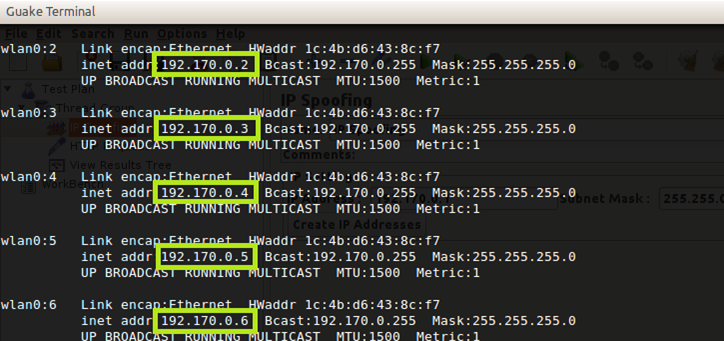
\includegraphics[width=12cm]{images/ips.png}
 \caption{Server records same IP for each virtual user}
\end{figure}
\end{frame}

%--------------------------------------------------------------------------------------
%               Slide 7
%--------------------------------------------------------------------------------------
\subsection{Server Response Without IP Spoofing}
\begin{frame}[c]
\frametitle{Server Response Without IP Spoofing}
\begin{figure}
 \centering
 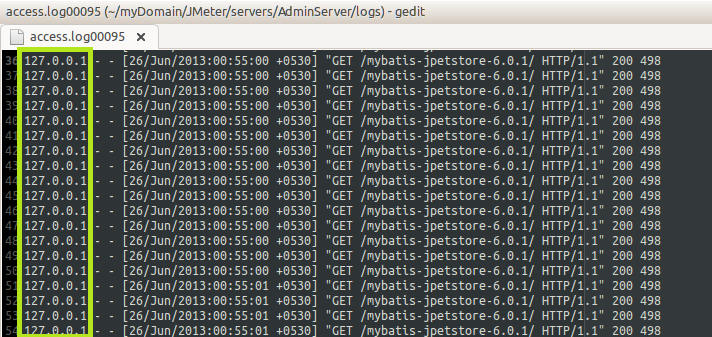
\includegraphics[width=12cm]{images/sl2.png}
 \caption{Server records same IP for each virtual user}
\end{figure}
\end{frame}

%--------------------------------------------------------------------------------------
%               Slide 8
%--------------------------------------------------------------------------------------
\subsection{Server Response With IP Spoofing}
\begin{frame}[c]
\frametitle{Server Response With IP Spoofing}
\begin{figure}
 \centering
 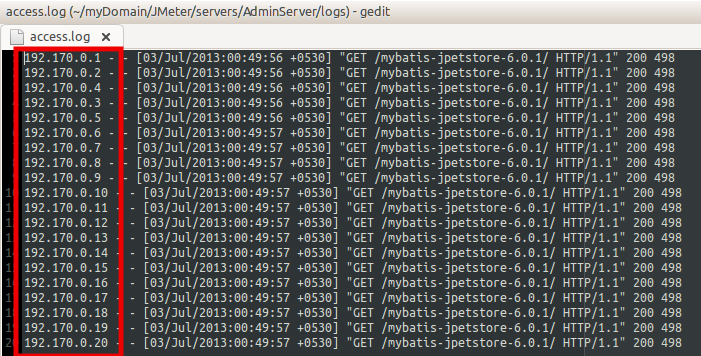
\includegraphics[width=12cm]{images/sl.png}
 \caption{Server records distinct IP for each virtual user}
\end{figure}
\end{frame}

%--------------------------------------------------------------------------------------
%               Slide 3
\section{Automating TPC-C Benchmarking}
\begin{frame}
 \begin{center}
    \FontviHead{Automating TPC-C Benchmarking}
 \end{center}

 
\end{frame}
%--------------------------------------------------------------------------------------
\section{Automating TPC-C Benchmarking}
\begin{frame}[c]
 \frametitle{Automating TPC-C Benchmarking}
\begin{itemize}
   \item<+-| alert@+>TPC- Transaction Processing Council
   It defines transaction processing and database benchmarks and delivers trusted results.
   \item <+-| alert@+> Some benchmarks undertaken under TPC:
   \begin{itemize}
    \item TPC-APP
    \item TPC-H
    \item TPC-C
   \end{itemize}

\end{itemize}

\end{frame}


%--------------------------------------------------------------------------------------
%               Slide 4
%--------------------------------------------------------------------------------------
\subsection{WHY TPC-C?}
\begin{frame}[c]
\frametitle{WHY TPC-C?}
%   \begin{block}{Block title 1}
%     text 1 \\ 
%     You can also insert numbered and bulleted list in this block \\ 
%     text 3 
%   \end{block}
%   \begin{block}{Output}
%     text 1 \\ 
%     text 2 \\ 
%     If it goes out of bound, create another slide.
%   \end{block}
\begin{itemize}
 \item A number of these benchmarks have been deprecated. TPC-C is currently in use and a rather complex process.
 \item A number of business houses use this benchmark to showcase their performance for OLTP transactions. It gives the measure of Server speed for online transaction processing.
\end{itemize}

\end{frame}

%--------------------------------------------------------------------------------------
%               Slide 4
%--------------------------------------------------------------------------------------
\subsection{}
\begin{frame}[c]
\frametitle{}
%   \begin{block}{Block title 1}
%     text 1 \\ 
%     You can also insert numbered and bulleted list in this block \\ 
%     text 3 
%   \end{block}
%   \begin{block}{Output}
%     text 1 \\ 
%     text 2 \\ 
%     If it goes out of bound, create another slide.
%   \end{block}
\begin{itemize}
 \item The actual benchmarking process is a time taking and a costly affair.
 \item A preliminary test would be a highly useful tool to test a server for performance and hence improve it where it lacks. 
\end{itemize}

\end{frame}

%--------------------------------------------------------------------------------------
%               Slide 4
%--------------------------------------------------------------------------------------
\subsection{The Benchmarking Model}
\begin{frame}[c]
\frametitle{The Benchmarking Model}
%   \begin{block}{Block title 1}
%     text 1 \\ 
%     You can also insert numbered and bulleted list in this block \\ 
%     text 3 
%   \end{block}
%   \begin{block}{Output}
%     text 1 \\ 
%     text 2 \\ 
%     If it goes out of bound, create another slide.
%   \end{block}
\centering
   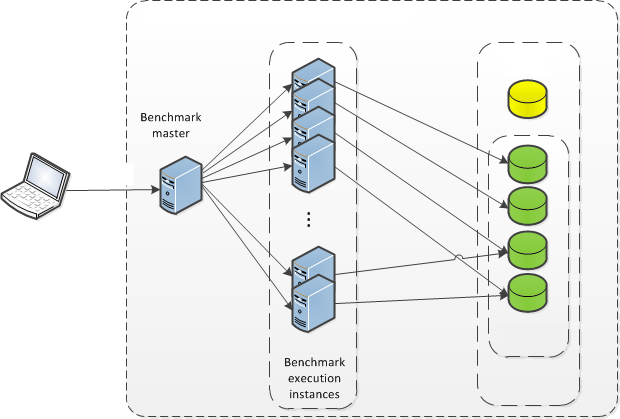
\includegraphics[width=10cm, height=7.5cm]{images/benchmarkmodel}

\end{frame}

%--------------------------------------------------------------------------------------
%               Slide 4
%--------------------------------------------------------------------------------------
\subsection{TPC-C Model}
\begin{frame}[c]
\frametitle{The Benchmarking Model}
%   \begin{block}{Block title 1}
%     text 1 \\ 
%     You can also insert numbered and bulleted list in this block \\ 
%     text 3 
%   \end{block}
%   \begin{block}{Output}
%     text 1 \\ 
%     text 2 \\ 
%     If it goes out of bound, create another slide.
%   \end{block}
The model emulated for TPC-C\\
\centering
   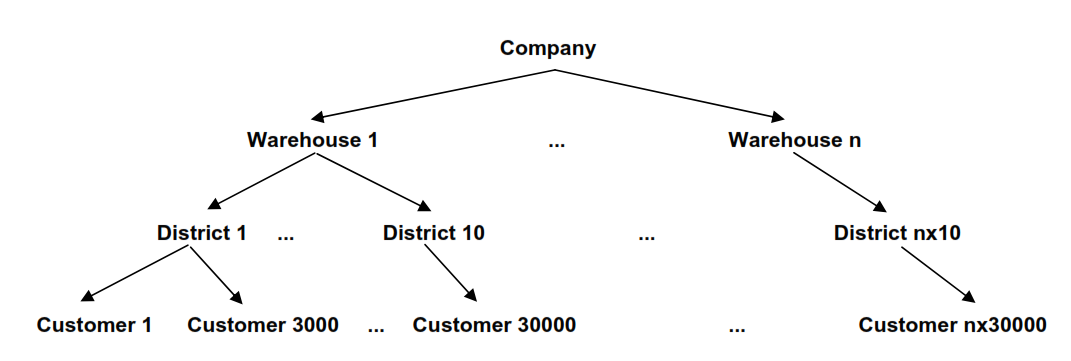
\includegraphics[width=10cm, height=4cm]{images/model}

\end{frame}

%--------------------------------------------------------------------------------------
%               Slide 4
%--------------------------------------------------------------------------------------
\subsection{Tables in the TPC-C schema}
\begin{frame}[c]
\frametitle{Tables in the TPC-C schema}
%   \begin{block}{Block title 1}
%     text 1 \\ 
%     You can also insert numbered and bulleted list in this block \\ 
%     text 3 
%   \end{block}
%   \begin{block}{Output}
%     text 1 \\ 
%     text 2 \\ 
%     If it goes out of bound, create another slide.
%   \end{block}
\begin{itemize}
 \item Item
 \item Warehouse
 \item History
 \item District
 \item Customer
 \item New Order
 \item Orders
 \item Order Line
 \item Stock
\end{itemize}

\end{frame}

%--------------------------------------------------------------------------------------
%               Slide 4
%--------------------------------------------------------------------------------------
\subsection{Transactions}
\begin{frame}[c]
\frametitle{Transactions}
%   \begin{block}{Block title 1}
%     text 1 \\ 
%     You can also insert numbered and bulleted list in this block \\ 
%     text 3 
%   \end{block}
%   \begin{block}{Output}
%     text 1 \\ 
%     text 2 \\ 
%     If it goes out of bound, create another slide.
%   \end{block}
\begin{itemize}
 \item New-order: enter a new order from a customer
 \item Payment: update customer balance to reflect a payment
 \item Delivery: deliver orders
 \item Order-status: retrieve status of customer’s most recent order
 \item Stock-level: monitor warehouse inventory
 
\end{itemize}

\end{frame}

%--------------------------------------------------------------------------------------
%               Slide 4
%--------------------------------------------------------------------------------------
\subsection{TPC-C Workflow}
\begin{frame}[c]
\frametitle{TPC-C Workflow}
%   \begin{block}{Block title 1}
%     text 1 \\ 
%     You can also insert numbered and bulleted list in this block \\ 
%     text 3 
%   \end{block}
%   \begin{block}{Output}
%     text 1 \\ 
%     text 2 \\ 
%     If it goes out of bound, create another slide.
%   \end{block}

\centering
   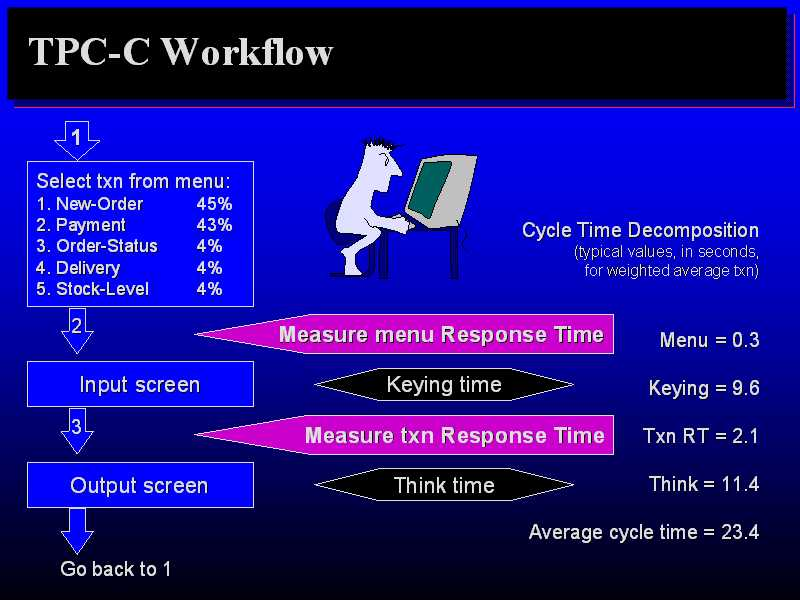
\includegraphics[width=10cm, height=7cm]{images/workflow}

\end{frame}

%--------------------------------------------------------------------------------------
%               Slide 4
%--------------------------------------------------------------------------------------
\subsection{Why JMeter to automate??}
\begin{frame}[c]
\frametitle{Why JMeter to automate??}
%   \begin{block}{Block title 1}
%     text 1 \\ 
%     You can also insert numbered and bulleted list in this block \\ 
%     text 3 
%   \end{block}
%   \begin{block}{Output}
%     text 1 \\ 
%     text 2 \\ 
%     If it goes out of bound, create another slide.
%   \end{block}
\begin{itemize}
 \item<+-| alert@+>JMeter is already capable of spawning a large number of virtual users to simulate the interaction of the real users with the system under test.
 \item<+-| alert@+>The firing of a request and measurement of response time as well as throughput is embedded in JMeter.
\end{itemize}

\end{frame}

%--------------------------------------------------------------------------------------
%               Slide 4
%--------------------------------------------------------------------------------------
\subsection{TPC-C Testing in JMeter}
\begin{frame}[c]
\frametitle{TPC-C Testing in JMeter}
%   \begin{block}{Block title 1}
%     text 1 \\ 
%     You can also insert numbered and bulleted list in this block \\ 
%     text 3 
%   \end{block}
%   \begin{block}{Output}
%     text 1 \\ 
%     text 2 \\ 
%     If it goes out of bound, create another slide.
%   \end{block}

\centering
   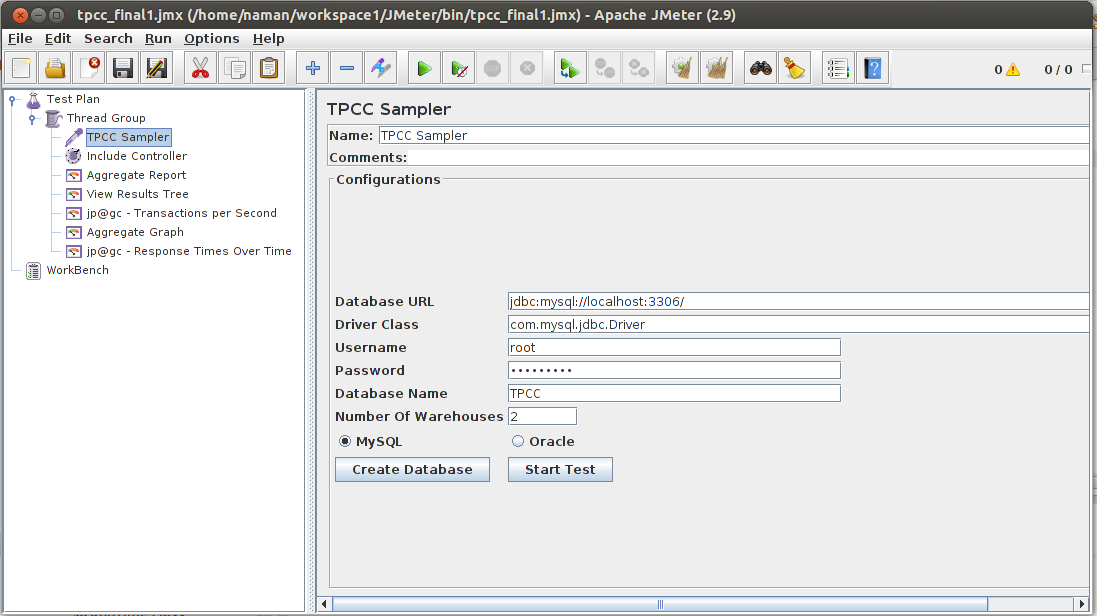
\includegraphics[width=11cm, height=6.5cm]{images/tpccgui1}

\end{frame}


%--------------------------------------------------------------------------------------
%               Slide 4
%--------------------------------------------------------------------------------------
\subsection{Controllers}
\begin{frame}[c]
\frametitle{Controllers}
Include Controller is a component of JMeter used to run saved scripts in JMeter.\\
%   \begin{block}{Block title 1}
%     text 1 \\ 
%     You can also insert numbered and bulleted list in this block \\ 
%     text 3 
%   \end{block}
%   \begin{block}{Output}
%     text 1 \\ 
%     text 2 \\ 
%     If it goes out of bound, create another slide.
%   \end{block}
\centering
   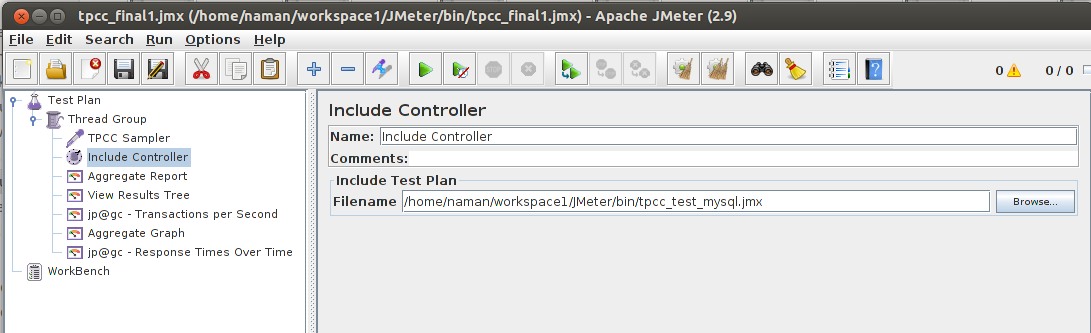
\includegraphics[width=9cm, height=5cm]{images/tpccgui2}

\end{frame}


%--------------------------------------------------------------------------------------
%               Slide 4
%--------------------------------------------------------------------------------------
\subsection{Test with 1 warehouse}
\begin{frame}[c]
\frametitle{Test with 1 warehouse}
%   \begin{block}{Block title 1}
%     text 1 \\ 
%     You can also insert numbered and bulleted list in this block \\ 
%     text 3 
%   \end{block}
%   \begin{block}{Output}
%     text 1 \\ 
%     text 2 \\ 
%     If it goes out of bound, create another slide.
%   \end{block}
\centering
   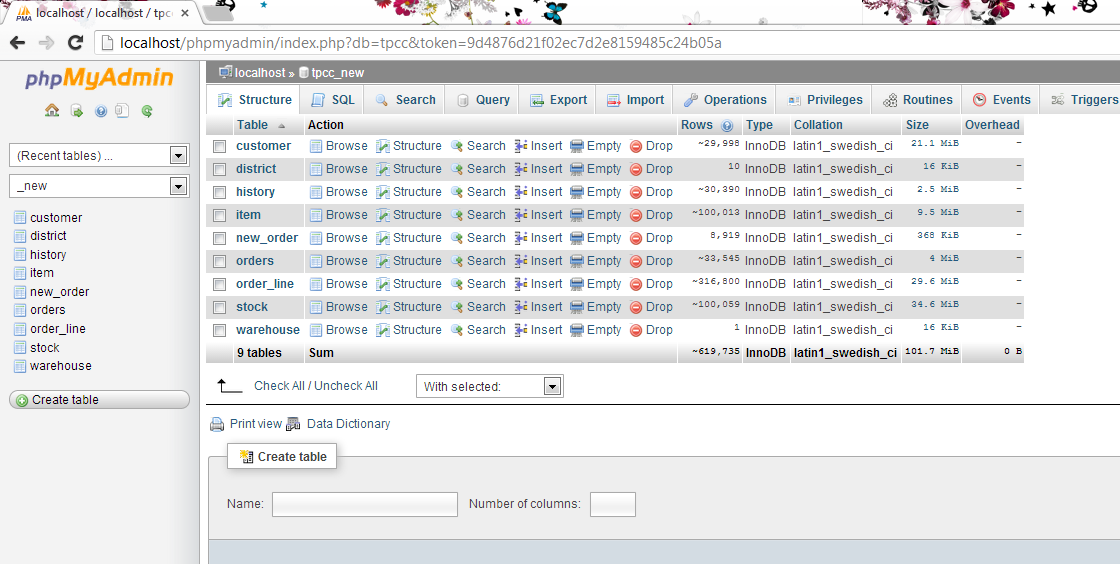
\includegraphics[width=11cm, height=7cm]{images/warehouse1}

\end{frame}

%--------------------------------------------------------------------------------------
%               Slide 4
%--------------------------------------------------------------------------------------
\subsection{Procedures}
\begin{frame}[c]
\frametitle{Procedures}
%   \begin{block}{Block title 1}
%     text 1 \\ 
%     You can also insert numbered and bulleted list in this block \\ 
%     text 3 
%   \end{block}
%   \begin{block}{Output}
%     text 1 \\ 
%     text 2 \\ 
%     If it goes out of bound, create another slide.
%   \end{block}
\centering
   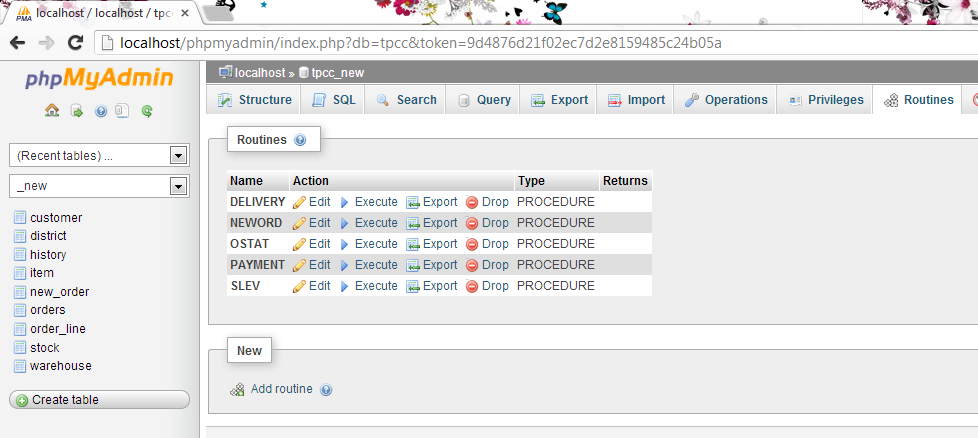
\includegraphics[width=11cm, height=5cm]{images/procedures}

\end{frame}

%--------------------------------------------------------------------------------------
%               Slide 4
%--------------------------------------------------------------------------------------
\subsection{Test with 33 Warehouses}
\begin{frame}[c]
\frametitle{Test with 33 Warehouses}
%   \begin{block}{Block title 1}
%     text 1 \\ 
%     You can also insert numbered and bulleted list in this block \\ 
%     text 3 
%   \end{block}
%   \begin{block}{Output}
%     text 1 \\ 
%     text 2 \\ 
%     If it goes out of bound, create another slide.
%   \end{block}
\centering
   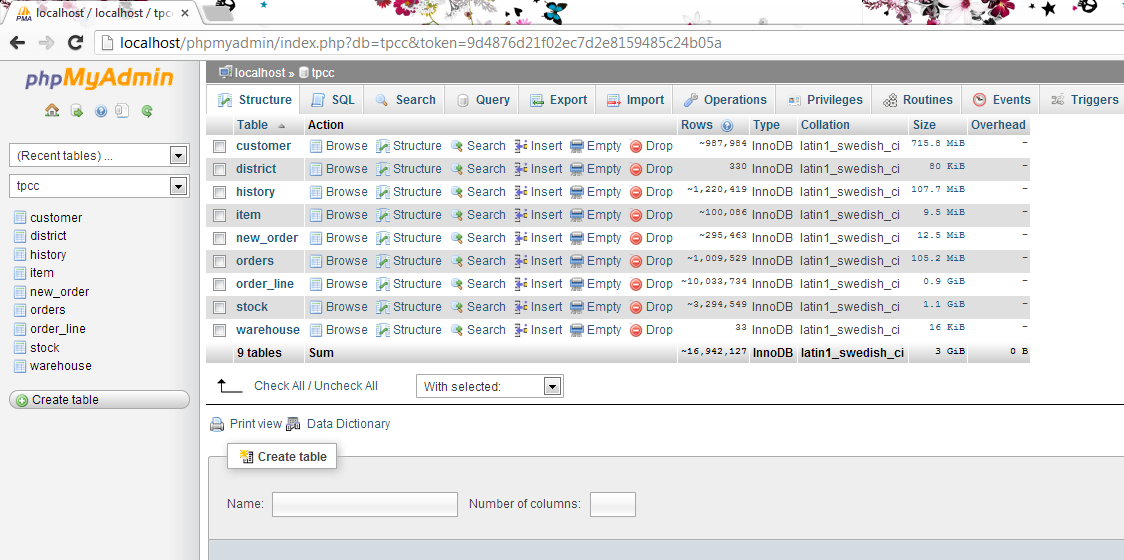
\includegraphics[width=11cm, height=7cm]{images/warehouse33}

\end{frame}


%--------------------------------------------------------------------------------------
%               Slide 4
%--------------------------------------------------------------------------------------
\subsection{JDBC Configuration}
\begin{frame}[c]
\frametitle{JDBC Configuration}
%   \begin{block}{Block title 1}
%     text 1 \\ 
%     You can also insert numbered and bulleted list in this block \\ 
%     text 3 
%   \end{block}
%   \begin{block}{Output}
%     text 1 \\ 
%     text 2 \\ 
%     If it goes out of bound, create another slide.
%   \end{block}
\centering
   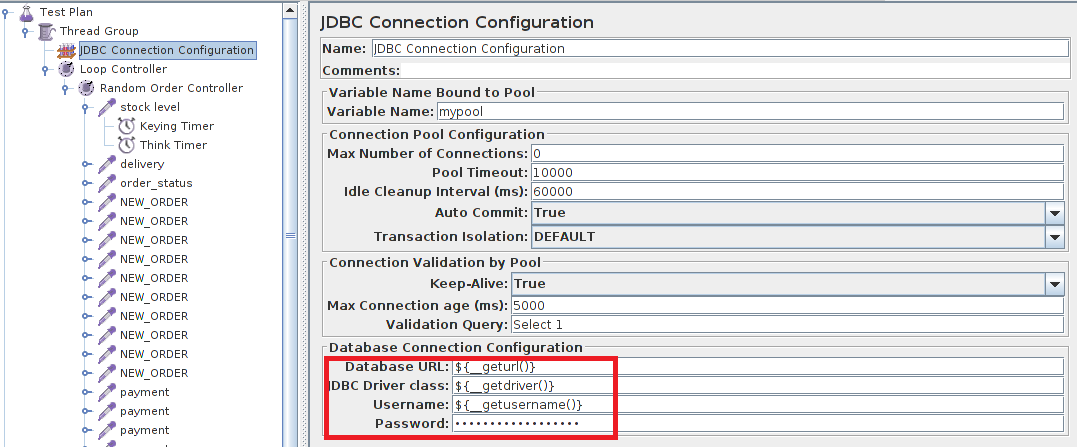
\includegraphics[width=11cm, height=6cm]{images/jdbcconfig}

\end{frame}

%--------------------------------------------------------------------------------------
%               Slide 4
%--------------------------------------------------------------------------------------
\subsection{Controllers}
\begin{frame}[c]
\frametitle{Controllers}
%   \begin{block}{Block title 1}
%     text 1 \\ 
%     You can also insert numbered and bulleted list in this block \\ 
%     text 3 
%   \end{block}
%   \begin{block}{Output}
%     text 1 \\ 
%     text 2 \\ 
%     If it goes out of bound, create another slide.
%   \end{block}
\centering
   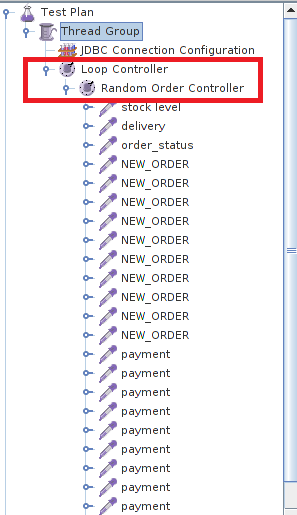
\includegraphics[width=5cm, height=6cm]{images/controller}

\end{frame}

%--------------------------------------------------------------------------------------
%               Slide 4
%--------------------------------------------------------------------------------------
\subsection{Timers}
\begin{frame}[c]
\frametitle{Timers}
%   \begin{block}{Block title 1}
%     text 1 \\ 
%     You can also insert numbered and bulleted list in this block \\ 
%     text 3 
%   \end{block}
%   \begin{block}{Output}
%     text 1 \\ 
%     text 2 \\ 
%     If it goes out of bound, create another slide.
%   \end{block}
\centering
   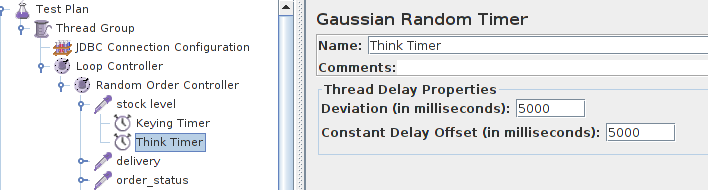
\includegraphics[width=8cm, height=4cm]{images/timer}

\end{frame}

%--------------------------------------------------------------------------------------
%               Slide 4
%--------------------------------------------------------------------------------------
\subsection{Transaction Call}
\begin{frame}[c]
\frametitle{Transaction Call}
%   \begin{block}{Block title 1}
%     text 1 \\ 
%     You can also insert numbered and bulleted list in this block \\ 
%     text 3 
%   \end{block}
%   \begin{block}{Output}
%     text 1 \\ 
%     text 2 \\ 
%     If it goes out of bound, create another slide.
%   \end{block}
\centering
   \includegraphics[width=12cm, height=7.7cm]{images/procedurecall}

\end{frame}

%--------------------------------------------------------------------------------------
%               Slide 4
%--------------------------------------------------------------------------------------
\subsection{Function Helper}
\begin{frame}[c]
\frametitle{Function Helper}
%   \begin{block}{Block title 1}
%     text 1 \\ 
%     You can also insert numbered and bulleted list in this block \\ 
%     text 3 
%   \end{block}
%   \begin{block}{Output}
%     text 1 \\ 
%     text 2 \\ 
%     If it goes out of bound, create another slide.
%   \end{block}
\centering
   \includegraphics[width=12cm, height=7.7cm]{images/functionhelper}

\end{frame}

%--------------------------------------------------------------------------------------
%               Slide 4
%--------------------------------------------------------------------------------------
\subsection{Procedure Request}
\begin{frame}[c]
\frametitle{Procedure Request}
%   \begin{block}{Block title 1}
%     text 1 \\ 
%     You can also insert numbered and bulleted list in this block \\ 
%     text 3 
%   \end{block}
%   \begin{block}{Output}
%     text 1 \\ 
%     text 2 \\ 
%     If it goes out of bound, create another slide.
%   \end{block}
\centering
   \includegraphics[width=10cm, height=5cm]{images/request}

\end{frame}


%--------------------------------------------------------------------------------------
%               Slide 4
%--------------------------------------------------------------------------------------
\subsection{Response}
\begin{frame}[c]
\frametitle{Response}
%   \begin{block}{Block title 1}
%     text 1 \\ 
%     You can also insert numbered and bulleted list in this block \\ 
%     text 3 
%   \end{block}
%   \begin{block}{Output}
%     text 1 \\ 
%     text 2 \\ 
%     If it goes out of bound, create another slide.
%   \end{block}
\centering
   \includegraphics[width=12cm, height=7cm]{images/response}

\end{frame}


%--------------------------------------------------------------------------------------
%               Slide 4
%--------------------------------------------------------------------------------------
\subsection{Aggregate Report}
\begin{frame}[c]
\frametitle{Aggregate Report}
%   \begin{block}{Block title 1}
%     text 1 \\ 
%     You can also insert numbered and bulleted list in this block \\ 
%     text 3 
%   \end{block}
%   \begin{block}{Output}
%     text 1 \\ 
%     text 2 \\ 
%     If it goes out of bound, create another slide.
%   \end{block}
\centering
   \includegraphics[width=12cm, height=7cm]{images/aggregate}

\end{frame}

%--------------------------------------------------------------------------------------
%               Slide 4
%--------------------------------------------------------------------------------------
\subsection{Transactions per second}
\begin{frame}[c]
\frametitle{Transactions per second}
%   \begin{block}{Block title 1}
%     text 1 \\ 
%     You can also insert numbered and bulleted list in this block \\ 
%     text 3 
%   \end{block}
%   \begin{block}{Output}
%     text 1 \\ 
%     text 2 \\ 
%     If it goes out of bound, create another slide.
%   \end{block}
\centering
   \includegraphics[width=12cm, height=7cm]{images/responseovertime}

\end{frame}


%--------------------------------------------------------------------------------------
%               Slide 4
%--------------------------------------------------------------------------------------
\subsection{Aggregate Graph}
\begin{frame}[c]
\frametitle{Aggregate Graph}
%   \begin{block}{Block title 1}
%     text 1 \\ 
%     You can also insert numbered and bulleted list in this block \\ 
%     text 3 
%   \end{block}
%   \begin{block}{Output}
%     text 1 \\ 
%     text 2 \\ 
%     If it goes out of bound, create another slide.
%   \end{block}
\centering
   \includegraphics[width=12cm, height=7cm]{images/aggregategraph}

\end{frame}

%--------------------------------------------------------------------------------------
%               Slide 4
%--------------------------------------------------------------------------------------
\subsection{Response Time over time}
\begin{frame}[c]
\frametitle{Response time over time}
%   \begin{block}{Block title 1}
%     text 1 \\ 
%     You can also insert numbered and bulleted list in this block \\ 
%     text 3 
%   \end{block}
%   \begin{block}{Output}
%     text 1 \\ 
%     text 2 \\ 
%     If it goes out of bound, create another slide.
%   \end{block}
\centering
   \includegraphics[width=12cm, height=7cm]{images/responsetime}

\end{frame}

%--------------------------------------------------------------------------------------
%               Slide 1a
%--------------------------------------------------------------------------------------
\section{Challenges}
\begin{frame}[c]
\frametitle{Challenges}
\begin{enumerate}
\item<+-|alert@+> Auto CSV Generation:
\\Generating CSV file for a particular table from a specified Database
\item<+-|alert@+> Dynamic Bandwidth Throttling:
\\Changing bandwidth in runtime and determining a reliable parameter (Percentage Error) to implement throttle bandwidth
\item<+-|alert@+> IP Spoofing:
\\Finding an array of un-used IPs and automating allocation of virtual IPs for a system
\item<+-|alert@+> Automating TPC-C testing:
\\Making tpcc testing capable of being run with different databases
  incroporating all the standards into JMeter
\end{enumerate}
\end{frame}

%--------------------------------------------------------------------------------------
%               Slide 2
%--------------------------------------------------------------------------------------
\section{Future Work}
\begin{frame}[c]
\frametitle{Future Work}
\begin{enumerate}
\item<+-|alert@+>  Incorporating other Benchmarking support such as TPC-H, TPC-E etc. into JMeter.
\item<+-|alert@+> Automation of the test scripts, as in user may not have to create the test script, and Jmeter can itself do it for the tester by techniques such as web crawling, etc.
\item<+-|alert@+>  The instability of JMeter on large loads could be worked out with some solution.
\item<+-|alert@+> Bringing large download efficiency into JMeter.
\item<+-|alert@+>  Better analysis of the results produced by JMeter via some complex graphs and better comparison between different graph results.
\end{enumerate}
\end{frame}

%--------------------------------------------------------------------------------------
%
%--------------------------------------------------------------------------------------

\section{Conclusion}
\begin{frame}[c]
 \frametitle{Conclusion}
 \begin{itemize}
  \item<+-|alert@+>The basic aim of the project was to enhance JMeter with the introduction of some new features and overcome some drawbacks.
  \item<+-|alert@+>We have made JMeter capable of performing more practical tests with the introduction of bandwitdh throttling and IP Spoofing.
  \item<+-|alert@+>The user friendliness of JMeter has been improved with the introduction of auto csv generation and results filtering.
  \item<+-|alert@+>Finally Jmeter has been extended from just a load testing tool to a Preliminary TPC-C benchmarking tool.

 \end{itemize}

\end{frame}

%--------------------------------------------------------------------------------------
%               Slide 7
%--------------------------------------------------------------------------------------
\section{References}
\begin{frame}[c]
\frametitle{References}
\bibliographystyle{ieeetr}
\beamertemplatetextbibitems
\FontviRef{
\bibliography{./biblio}
}
\end{frame}



%--------------------------------------------------------------------------------------
%               Slide 8
%--------------------------------------------------------------------------------------
%--------------------------------------------------------------------------------------
%               Slide 3
%--------------------------------------------------------------------------------------
\section{Educational Application}
\begin{frame}[c]
\frametitle{Educational Application}
\begin{block}{Learning Shapes}
 \begin{columns}[c]
  \column{0.4\textwidth}
   \includegraphics[width=5cm]{images/screen1.png}
  \column{0.5\textwidth}
A simple application to teach young minds the sense of shapes and colors. This app tests the recognition skill shapes and colors among children
 \end{columns}
\end{block}

\begin{block}{Traingles for High School}
 \begin{columns}[c]
  \column{0.4\textwidth}
   \includegraphics[width=5cm, height=2.5cm]{images/screen2.png}
  \column{0.5\textwidth}
An application to aid learning about Triangles, allows construction of Triangles, also drawing Triangles from user Input
\end{columns}
\end{block}
\end{frame}

\begin{frame}[c]
\frametitle{Educational Application}
\begin{block}{Mathematics Playground}
 \begin{columns}[c]
  \column{0.4\textwidth}
   \includegraphics[width=5cm]{images/screen3.png}
  \column{0.5\textwidth}
Best friend of any student during examination for quick revision of the formulas.The detailed proofs and animation helps the student in recalling the logic behind the formula
 \end{columns}
\end{block}

\begin{block}{Base Conversion}
 \begin{columns}[c]
  \column{0.4\textwidth}
   \includegraphics[width=5cm]{images/screen4.png}
  \column{0.5\textwidth}
This application teaches Base Conversion, it describes the conversion procedure from any positive integral base to any other positive integral base
 \end{columns}
\end{block}
\end{frame}

\begin{frame}[c]
\frametitle{Educational Application}
\begin{block}{Area of Polygons}
 \begin{columns}[c]
  \column{0.4\textwidth}
   \includegraphics[width=5cm]{images/screen5.png}
  \column{0.5\textwidth}
This application teaches methods to calculate area of any Polygon. Polygon is drawn by user input and area is calculated and displayed with explanation
 \end{columns}
 \end{block}
 
 \begin{block}{Currency Converter}
 \begin{columns}[c]
  \column{0.4\textwidth}
   \includegraphics[width=5cm, height=2.5cm]{images/currency}
  \column{0.5\textwidth}
   This application provides the methods of currency conversion as well as the details of the country to which the currency belongs.
 \end{columns}
\end{block}


\end{frame}

\section{Team Members}
\begin{frame}
 \frametitle{Enhancement of JMeter - Team Members}
  \hspace{0.5cm}\includegraphics[width=2cm, height=2cm]{images/sushmitha}\hspace{1.5cm}
  \includegraphics[width=2cm, height=2cm]{images/dhruv}\hspace{1.5cm}
  \includegraphics[width=2cm, height=2cm]{images/manisha}\\
  B. Sushmitha\hspace{1.5cm} 	Dhruv Joshi \hspace{1.5cm} Manisha Choudhury\\
  \vspace{0.5cm}
  \hspace{0.5cm}\includegraphics[width=2cm, height=2cm]{images/naman}\hspace{1.5cm}
  \includegraphics[width=2cm, height=2cm]{images/shekhar}\hspace{1.5cm}
  \includegraphics[width=2cm, height=2cm]{images/surabhi}\\
  Naman Choudhary \hspace{0.5cm} Shekhar Saurav \hspace{0.5cm} Surabhi Mour
  
\end{frame}


\end{document}
